\section{What the brain does for an agent: the tests}\label{sec:tests}

\subsection{Protocol}
Every test below compares arms that differ only in access to the brain, with one exception: the layered solving test of Section~\ref{subsec:solve61}, whose fifth layer adds a clock and a hint along with the held notes. The arms use the same model, the same reasoning setting, the same budget of time and tokens, the same tools apart from the brain's, and the same items, and each item is worked by a fresh session so that no arm learns from another. An item is scored correct or incorrect against a private key by a grader that does not see which arm produced the answer. For two arms $A$ and $B$ on the same items, let $n_{AB}$ be the number of items $A$ answered and $B$ did not, and $n_{BA}$ the reverse. The exact two-sided McNemar $p$-value is
\[
p=\min\Bigl(1,\ 2\sum_{j=0}^{\min(n_{AB},n_{BA})}\binom{n_{AB}+n_{BA}}{j}2^{-(n_{AB}+n_{BA})}\Bigr).
\]
We report $n_{AB}$ to $n_{BA}$ beside every $p$. The values quoted were recomputed from the counts by a script included with the paper.

Before reporting a null result we compute the test's room to fail: how many items the better arm could have lost, and whether the instrument could have seen the effect in question. A test in which one arm is already perfect cannot show that arm improving, and its $p$-value says nothing about the brain.

\subsubsection*{Contamination}
The answer to a recall question is, by construction, a card in the store, so the store must not contain the question, its key or an earlier answer to it. Every evaluation passes a retrieval guard that removes, before scoring, every record outside the allowed splits, every answer key, solution, fault annotation and prior evaluation output, the active item and its paired variants, and any record sharing a prohibited source digest. Test sessions are not logged into the link strengths (Section~\ref{sec:strength}). The question banks themselves are kept off the store and out of every repository, so that the same tests can be run on later versions without the answers having been seen. One contamination we cannot rule out is the model's own training data: the arm without the brain may know a published result from pre-training. For published material this is an uncertainty whose direction depends on the outcome measured; for the agents' own results, which were never published before the tests, it does not arise. A second limitation is adaptive: the banks were also used to decide whether packets and ranking changes land, so a result on a bank that informed such a decision is weaker than one on a holdout that no decision touched. The ranking test below was scored on questions held out from its own tuning, but the other banks were reused, and the main comparisons would be stronger on a final holdout that no decision has touched.

\subsection{Three arms on a thousand items}\label{subsec:threearm}
The largest test compares three arms and nothing else. In the first the agent has the brain: the recall tool, served without a shell, and the two prompt hooks of Section~\ref{sec:hook}, and no file tools. In the second it has no brain, no hooks and no recall tool, but it can read, list and search the research repositories, which include the exported store, the campaign records and the open-problem files; the brain's own folders, its transcripts, the keys and every test folder are denied to it. In the third it has the model alone, with no tools. Every arm sees the same system text, the same instructions on how to answer and the same item, one item a session. Claude Sonnet agents (high reasoning) had $600$ seconds an item and Codex agents (gpt-6.1-sol, high reasoning) $900$ seconds. No Claude arm had a shell. For Codex the brain arm had the recall tool and the hook notes and no shell, the documents arm a read-only shell over the same repositories, and the third arm nothing. The runs took place on 23 and 24 October 2026. The Claude run splits the bank into three shards run side by side, and the Codex run takes items the Claude run has already finished; the figures below cover the items that had been run in all three arms by the evening of 24 October, $755$ of the $1{,}000$ for Claude and $182$ for Codex.

The bank was built on 12 September 2026 and has $1{,}000$ items. $923$ are lookups over the store's records: questions on the open-problem ledger (the sum or the difference of the pages on which listed problems are posed in their sources, which of four is posed latest, which source is the odd one out) and on the self-avoiding-walk counts held in the store, each combining two to four records. The other $77$ are proof audits, in which the agent decides whether a numbered proof is correct as written and, if not, names its first invalid step. The lookups test what the memory is for; the audits are a mathematics control, since their answers are not stored anywhere. A timeout or an error without an answer counts as wrong. A session that never reached the model (a refused account or a session limit, recognised by an empty event stream) is dropped and rerun, not graded.

\begin{table}[ht]
\centering\small
\begin{tabular}{llccc}
\toprule
 & & Brain & Documents & No tools\\
\midrule
Claude, $755$ items run in all arms & correct & $94.3\%$ & $78.1\%$ & $21.7\%$\\
 & sessions timed out & $4.8\%$ & $21.2\%$ & $35.8\%$\\
 & mean seconds an item & $136$ & $241$ & $249$\\
Claude, $593$ items both brain and documents & correct & $99.2\%$ & $99.3\%$ & \\
\quad answered in time & & & & \\
Claude, $480$ items all arms answered in time & correct & $99.2\%$ & $99.4\%$ & $34.0\%$\\
\quad of which proof audits, $68$ & correct & $98.5\%$ & $97.1\%$ & $98.5\%$\\
Codex, $182$ items run in all arms & correct & $93.4\%$ & $97.3\%$ & $31.9\%$\\
\quad of which proof audits, $50$ & correct & $98.0\%$ & $94.0\%$ & $92.0\%$\\
\bottomrule
\end{tabular}
\caption{The three-arm test, Claude Sonnet and Codex gpt-6.1-sol, 24 October 2026. ``Documents'' is the arm with the repositories and no brain.}
\label{tab:threearm}
\end{table}

For Claude the brain beat the documents $134$ to $12$ on the items where they disagreed ($p=3.0\cdot10^{-27}$) and the bare model $549$ to $1$; the documents beat the bare model $427$ to $1$. The first of these numbers needs reading with the rest of the table. On the $593$ items that the brain arm and the documents arm both answered within the time, they are tied, $99.2\%$ against $99.3\%$, $2$ to $3$. The brain's lead over the documents is therefore almost entirely time: an agent searching the files finds the same records, but it needs more searches to find them, and on about a fifth of the items it is still searching when the clock runs out. The gap is largest on the walk lookups that need three or four records, where the documents arm answered $31$ to $51\%$ of the items in a family and the brain arm $76$ to $95\%$. All but one of the bare model's timed-out sessions fall on these walk lookups, where it tries to enumerate the walks by hand.

The Codex agents had half again as much time and seldom ran out of it. There the documents arm scored $97.3\%$ against $93.4\%$ for the brain ($3$ to $10$, $p=0.09$; on the lookups alone $1$ to $10$, $p=0.012$, which does not survive the correction of Appendix~\ref{app:stats}). On the first $100$ Codex items every one of the brain arm's losses was an abstention, never a wrong value. In two the agent never called the recall tool. In three its searches missed records that the documents arm found by reading the files; in one of these the record held a string of punctuation and digits, which the recall tool's lexical match handles poorly and a text search finds at once. Neither aid moved the proof audits, which every arm, the bare model included, answered at about the same rate: the store adds nothing to a proof that the model can check by itself.

\subsubsection*{What it cost}
The $923$ lookups were generated by scripts from the store's records, and every key was derived twice, from separate reads, with no disagreement. The $77$ proof audits were written by Claude Opus~5 agents on 12 September 2026 and each key was confirmed by a separate verifier; by the workflow's own record that took $2.3$ million tokens and $32$ minutes. The record keeps the total but not its split between input and output, so the price can only be bounded: at list price, \$5 a million input tokens and \$25 a million output tokens, it lies between \$12 and \$58, and cached input would bring it lower. Table~\ref{tab:threearm-cost} gives the cost of every session of the three-arm runs, timeouts and reruns included. The prices are those the Claude command-line client reports at list price; the runs used subscription accounts, and the Codex client reports no price. A session stopped at its time limit records neither tokens nor a price, so the token and price columns leave out the timed-out sessions.

\begin{table}[ht]
\centering\small
\begin{tabular}{llrrrrr}
\toprule
 & Arm & Sessions & Hours & \multicolumn{2}{c}{Tokens a session} & Price a\\
\cmidrule(lr){5-6}
 & & & & in & out & session\\
\midrule
Claude & brain & $808$ & $30.6$ & $20{,}000$ & $1{,}500$ & \$0.053\\
 & documents & $808$ & $53.2$ & $80{,}000$ & $4{,}000$ & \$0.092\\
 & no tools & $807$ & $54.8$ & $2{,}000$ & $300$ & \$0.010\\
Codex & brain & $227$ & $27.6$ & $45{,}000$ & $400$ & ---\\
 & documents & $231$ & $17.0$ & $57{,}000$ & $600$ & ---\\
 & no tools & $232$ & $14.8$ & $7{,}000$ & $3{,}100$ & ---\\
\bottomrule
\end{tabular}
\caption{Cost of the three-arm runs to 24 October 2026: $3{,}113$ sessions, $198$ session-hours, $107$ million input tokens, $5.7$ million output tokens, and \$125.69 at list price for the Claude sessions.}
\label{tab:threearm-cost}
\end{table}

With Claude the brain arm read a quarter of the documents arm's input, wrote two fifths of its output and used $58\%$ of its session-hours. Counting only the sessions that recorded a price, it cost $58\%$ as much a session; the documents arm's timed-out sessions, four times as many as the brain arm's, are left out of that figure, so the true ratio is probably lower. With Codex the order of the hours is reversed: on the graded sessions the brain arm took $244$ seconds an item against $215$, and its total includes sessions rerun after the connection to the recall server dropped.


\subsection{Recall of results held in the store}
One hundred questions each ask for a fact held in exactly one card. Sixty were reworded so that they share no content word with their card; forty are plain. Codex agents (gpt-6.1-sol, high reasoning) took one question per session. Table~\ref{tab:recall100} gives the five arms.

\begin{table}[ht]
\centering\small
\begin{tabular}{lc}
\toprule
Arm & Correct of 100\\
\midrule
no tools & 0\\
the hook's served notes, no tools & 7\\
text search over a copy of the store's files & 75\\
recall tool (whole cards, identifiers, linked identifiers) & 83\\
hook, recall tool and link walk (the full stack) & 82\\
\bottomrule
\end{tabular}
\caption{Recall of results held in the store, 11 October 2026.}
\label{tab:recall100}
\end{table}

The full stack against the recall tool alone went $2$ to $3$ ($p=1$). This is an estimate of a difference near zero, not a demonstration of equal accuracy: $17$ questions were wrong under the recall tool alone, so there was room for a gain, but a test of this size detects only a large one (Appendix~\ref{app:stats}: at $100$ items and a disagreement rate of $0.2$, power $0.8$ needs a net gain of about $13$). Against text search the full stack went $10$ to $3$ ($p=0.092$). With no tools the agents answered nothing: these are facts that exist only in the store.

The format of the printout decided much of the score. The same retrieval printing titles and $700$-character snippets without identifiers scored $34$; printing identifiers, whole cards and linked identifiers scored $83$.

Cost was measured from the session logs (Table~\ref{tab:recall-cost}). About $98\%$ of all input tokens were cached re-reads of the session, so the saving in uncached input is a factor of $1.8$, not $7.6$. On the first $20$ questions, with the same search tool in both arms, both scored $18$ of $20$; with the walk the sessions read $3.1$ million tokens and made $40$ searches, without it $16.9$ million tokens and $55$ searches. Unlike the rest of the test, these twenty questions were worked in two long sessions an arm rather than one question a session, so the size of that saving is uncertain.

\begin{table}[ht]
\centering\small
\begin{tabular}{lcc}
\toprule
 & Recall tool alone & Hook, recall and walk\\
\midrule
Input tokens, all questions & 186 million & 24.6 million\\
Uncached input tokens per question & 24 thousand & 13 thousand\\
Output tokens per question & 1.9 thousand & 0.4 thousand\\
Session-minutes, all questions & 666 & 78\\
\bottomrule
\end{tabular}
\caption{Cost of the two strongest arms of Table~\ref{tab:recall100}.}
\label{tab:recall-cost}
\end{table}

\subsection{Several wordings}
On a further $100$ held-out questions, the recall tool given two or three wordings of each question in one call answered $86$; given one wording a call (the agent free to call again) it answered $76$. Merged wordings were also the cheapest of the strong strategies, because each call is a turn that re-reads the whole session.

\subsection{Recall that the agent cannot do without the store}
On $13$ September agents answered $1{,}000$ items, each of which requires a fact that is a card in the store. Without the brain they answered $538$; with it, all $1{,}000$. The brain helped on $462$ items, and no harm was observed ($p=1.7\cdot10^{-139}$). The design did not exclude harm; the arm with the brain happened to be perfect, so what the test shows is the size of the gap the store closes on material of its own. It says nothing about reasoning items, which the solving tests below address.

\subsection{Ranking on held-out questions}
This test measures the retrieval engine without an agent: how often the answer card is among the first eight results, on questions that played no part in tuning. On 12 October the ranking was changed from the base profile to the recall profile of Section~\ref{sec:retrieval} after tuning on a development set.

\begin{table}[ht]
\centering\small
\begin{tabular}{lccc}
\toprule
 & Before & After & Gained to lost ($p$)\\
\midrule
584 held-out questions & 298 & 317 & 27 to 8 ($0.0019$)\\
six further sets, 1{,}070 questions & 891 & 1{,}018 & 143 to 16 ($1.1\cdot10^{-26}$)\\
\bottomrule
\end{tabular}
\caption{Answer card in the first eight results, before and after the ranking change of 12 October.}
\label{tab:ranking}
\end{table}

The six further sets moved unevenly: three gained $32$, $44$ and $66$; two that were already near the ceiling with word search alone lost $9$ and $7$; one gained $1$. The ranking was tuned on questions written by Codex agents, and its largest held-out gain is on a set written by Claude agents, which argues against overfitting to one author's phrasing. The gain comes from the ranking, BM25 with $b=0.4$ and titles counted twice; the meaning channel adds about nothing on these sets. On the development check the first-place hits rose from $37$ to $54$ of $142$ and the mean reciprocal rank from $0.331$ to $0.442$.

A proposed embedding of whole cards, built later, put the answer in the first eight for $52$ of $80$ questions against $27$ for the live channel. It has not been switched on, because it has not yet passed the held-out recall gate on the full sets.

\subsection{Files in GitHub repositories}
Questions were drawn from little-known files in GitHub repositories that the store indexes, and Codex agents (gpt-6.1-sol, medium reasoning) answered them with git, with and without the brain. A crash cut the run short. With git and the brain the agents answered $83$ of $90$ correctly; with git alone, $76$ of $90$. Both arms completed the same $80$ questions before the crash, and on those the scores were $73$ and $68$ ($9$ to $4$, $p=0.27$). The brain arm read $14\%$ more tokens per question. When the files are at hand, the brain adds little.

\subsection{Solving and auditing}\label{subsec:solve61}
Sixty-one items, from four pooled runs on 5 and 6 October, asked Claude Sonnet agents to solve a problem or to find the fault in a purported solution, with Python, Lean and file tools and up to $600$ seconds an item. The arms add one layer at a time: tools only; documents; ranked recall; the hook and the recall tool; held notes, a six-minute clock and a hint; and the statement of any named result the item refers to. The full package has every layer.

\begin{table}[ht]
\centering\small
\begin{tabular}{lcccc}
\toprule
Comparison & Items & Scores & Disagreements & $p$\\
\midrule
full package against tools only & 61 & 52 and 41 & 15 to 4 & 0.019\\
the same, without 7 items whose keys proved ambiguous & 54 & 48 and 39 & 12 to 3 & 0.035\\
items that name a known result & 26 & 22 and 13 & 10 to 1 & 0.012\\
items that name none & 35 & 30 and 28 & 5 to 3 & 0.73\\
full package against documents and recall & 61 & 52 and 46 & 10 to 4 & 0.18\\
\bottomrule
\end{tabular}
\caption{Solving and auditing, 5--6 October 2026.}
\label{tab:solve61}
\end{table}

The gain over tools alone is significant at $p=0.019$ as a single comparison but does not survive a Holm correction over all the paired comparisons of this paper (Appendix~\ref{app:stats}), and the full package changes more than the memory: its fifth layer adds a clock and a hint. Within it, the gain lies in the items that name a known result: an agent that is told, correctly, what a cited theorem says catches a misuse of it that an agent working from its own memory misses. Against agents that already have the documents and a recall tool, the further gain is not significant. Served notes cut both ways here. They helped on faults that drop a hypothesis, and they hurt on faults of citation, scope and sharpness, where a note about the cited result made a wrong use of it look legitimate; that observation is the reason for the trust line of Section~\ref{sec:hook}.

\subsection{What did not help}

\subsubsection*{Spreading activation}
Agents told why each card came up scored $79$ with spreading and $80$ without, while reading $46\%$ more input tokens. Without agents, on the $584$ questions, spreading moved first-eight hits from $298$ to $307$ but found no card the word search had missed: it re-ranks and nothing more. It is off by default.

\subsubsection*{A pointer to the next card}
A line printed under the cards, naming the card most often reached next from them, was tested on 15 October. Without agents it changed no ranking on the $584$ held-out questions, lost no answer, and on $6$ of them named an answer card that the printout showed nowhere else. Codex agents (gpt-6.1-sol, medium reasoning, ten questions a session) then answered $60$ further held-out questions, $30$ hard and $30$ plain, under three printouts of the recall tool: the printout of before 12 October, the current one, and the current one with the line. They answered $48$, $48$ and $45$ correctly ($28$, $28$ and $26$ of the hard questions). Against the current printout the line went $0$ to $3$ ($p=0.25$), and one of the three losses gives the right number in another notation; the agents opened $7$ of the $220$ cards the line named. The current printout against the earlier one went $2$ to $2$ ($p=1$) and read $16\%$ less uncached input a question ($10.1$ against $12.0$ thousand tokens). The $18$ sessions read $52$ million input tokens, $96\%$ of them cached re-reads, and wrote $75$ thousand. The line was not adopted. All three arms ran with the agents' ordinary start-up hooks, so their level is not comparable with Table~\ref{tab:recall100}, and at $60$ questions the test sees only a large effect.

\subsubsection*{New open problems}
Fourteen Codex agents worked $13$ open problems on which the store held only a first attempt, written in September. Each attempt was graded blind at up to $3$ points. The arm with the brain scored $24$ of $39$ and the arm without it $26$; a referee comparing each pair preferred the attempt without the brain $8$ times and the one with it $3$ times, with $2$ even ($p=0.23$). The store held almost nothing on these problems beyond a first attempt, so this test measures what the brain adds when it has little to recall, and the answer is nothing measurable. It does not measure the case for which the brain was built, a problem on which earlier agents have left many results.

\subsubsection*{An early version against plain documents}
On a hard set of $300$ items with no tools, version $1$ of the system (hook notes, the recall tool, Lean and an audit step) scored $238$, and agents given the documents directly scored $264$ ($14$ to $40$, $p=0.0005$). Most of the loss was in one group of $70$ items, $22$ against $55$, where the version-$1$ hook served notes that pulled agents off the documents. The later version, which routes to deliberate recall first, adds a clock and silences the hook on weak matches, was built in response to this result. On 4 October that version (lookup in the store first, Lean at most once with a limit of $90$ seconds, a $360$-second clock), run by Claude Sonnet agents on $110$ problems answerable from the store, scored $102$ against $104$ for agents given the documents and a recall tool ($6$ to $8$, $p=0.79$). The items and the baseline differ from those of the $300$-item run, so the two results do not form a before-and-after pair; the second shows neither a loss nor a gain against documents with recall.

\subsection{Deliberate recall over time}
The deliberate recall path was itself improved by the tests. On a fixed set of $64$ questions on the agents' own past work, the answer was first for $24$ questions in September and for $46$ after the changes described in Sections~\ref{sec:retrieval}--\ref{sec:hook}. On a larger held-out set the recall tool answered $317$ of $584$, against $298$ before the ranking change.

\begin{figure}[ht]
\centering
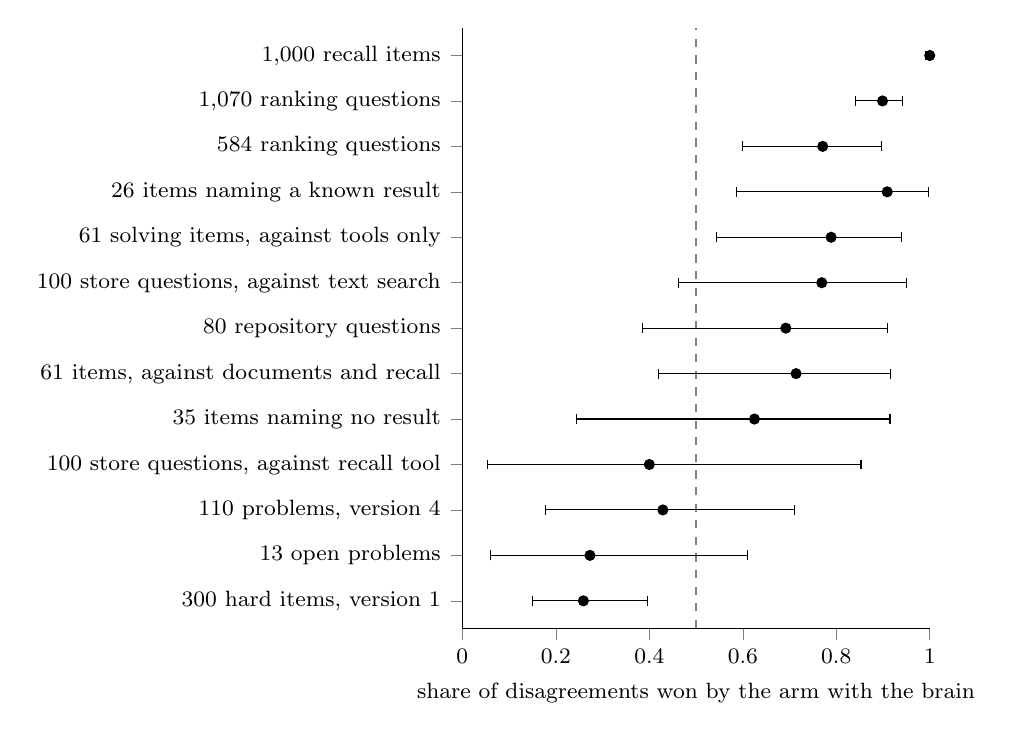
\begin{tikzpicture}
\begin{axis}[
  width=0.62\textwidth, height=9.2cm,
  xmin=0, xmax=1, ymin=0.4, ymax=13.6,
  xlabel={share of disagreements won by the arm with the brain},
  ytick={1,...,13},
  yticklabels={
    {300 hard items, version 1},
    {13 open problems},
    {110 problems, version 4},
    {100 store questions, against recall tool},
    {35 items naming no result},
    {61 items, against documents and recall},
    {80 repository questions},
    {100 store questions, against text search},
    {61 solving items, against tools only},
    {26 items naming a known result},
    {584 ranking questions},
    {1{,}070 ranking questions},
    {1{,}000 recall items}},
  yticklabel style={font=\footnotesize},
  xticklabel style={font=\footnotesize},
  xlabel style={font=\footnotesize},
  tick align=outside, axis x line*=bottom, axis y line*=left,
]
\addplot[gray, dashed] coordinates {(0.5,0.4) (0.5,13.6)};
\addplot[only marks, mark=*, mark size=1.8pt, black,
  error bars/.cd, x dir=both, x explicit]
  table[x=s, y=y, x error minus=m, x error plus=p] {
  y  s      m      p
  1  0.259  0.109  0.138
  2  0.273  0.213  0.337
  3  0.429  0.252  0.282
  4  0.400  0.347  0.453
  5  0.625  0.380  0.290
  6  0.714  0.295  0.202
  7  0.692  0.306  0.217
  8  0.769  0.307  0.181
  9  0.789  0.245  0.150
  10 0.909  0.322  0.089
  11 0.771  0.172  0.125
  12 0.899  0.057  0.042
  13 1.000  0.008  0.000
  };
\end{axis}
\end{tikzpicture}
\caption{The comparisons of the brain against a baseline on one scale: the share of the disagreeing items won by the arm with the brain, with an exact $95\%$ Clopper--Pearson interval. The dashed line is no effect. The four lowest rows are tests on which the brain did not help; the rows for versions~1 and~4 concern earlier versions on item sets and baselines of their own, and the open-problems row is a referee's pairwise preference. Intervals that cross the line are inconclusive, not evidence of equal accuracy.}
\label{fig:effects}
\end{figure}


\subsection{What the tests say}
Figure~\ref{fig:effects} puts the comparisons of the brain against a baseline on one scale, the losses and the inconclusive results included. The pattern across tests is consistent. The brain helps when the answer is something the agent cannot know: a result in the store and nowhere else ($538$ to $1{,}000$), or, less firmly, a cited theorem whose exact statement decides whether a proof is right ($13$ to $22$, a subset result that does not survive the correction for several comparisons). It saves cost when the agent can move along links instead of searching again (uncached input fell by a factor of $1.8$, with $82$ and $83$ correct). When the agent already has the documents and enough time, it finds the same records, and the brain adds speed and lower cost rather than accuracy: the three-arm test tied on the items both arms finished, and under a ten-minute limit that speed separated $94\%$ from $78\%$. It adds nothing measurable on a new problem about which the store knows nothing. The size of the effect is set by what is in the store, which is why the store's growth and the write-back path matter as much as the retrieval.

\subsection{The test bank}
The tests draw on a private bank of items written for the purpose. On 22 October $6{,}778$ items had been written and $256$ admitted. An item is admitted only after two independent audits agree that its key is correct and unambiguous, that it is answerable from the store for the recall strata, and that it is not answerable from the public files of the release (seventeen items answerable from the release files were retired). Admission is the bottleneck, not writing: most items fail on key repair, not on the audits. The bank, its keys and the per-item records are not published; anchors committing to the content of the blinded experiments are public, so that a later reader can check that the reported items were fixed before the runs.
